\subsection{Classification}
\subsubsection{Tree-walk kernel}

\begin{figure}[htb!]
\centering
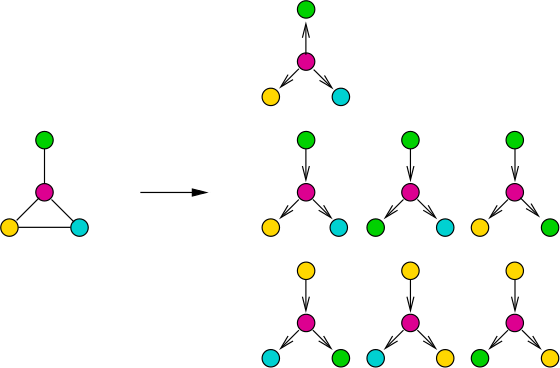
\includegraphics[width=0.7\textwidth]{images/treewalk.png}
\caption{Examples of tree walks in a graph, from the original paper \cite{harchaoui2007image}.}
\end{figure}

Our initial idea for classifying the animation characters is to consider the region adjacency graph on the segments of the image. The intuition is that although changes in posture, scale change the overall image significantly, the arrangement of segments in the image relative to each other should roughly stay the same. Classifying images by their region adjacency graph has been studied by Z. Harchaoui and F. Bach in \cite{harchaoui2007image}, in which they a introduce a number of kernels to compute similarity between such graphs. We chose to study and implement the tree-walk kernel presented in this paper.

\paragraph{The method} Let $I$ be a color image, $S = \{S_1, ..., S_q\}$ a segmentation of $I$ and a $4$-connected notion of adjacency between pixels. The region adjacency graph $G$ of $I$ is defined as the graph where vertices are segments and there is an edge between segments $S_i$ and $S_j$ if and only if there is a pair of adjacent pixels $(p_i, p_j) \in S_i \times S_j$.

Let $G$ and $H$ be region adjacency graphs with labelling functions $l_g : V(G) \rightarrow L$ and $l_h : V(H) \rightarrow L$, where $L$ is a segment label set. The method considers a kernel function $k : L \times L \rightarrow \mathbb{R}^+ \cup \{0\}$ which measures similarity between segment labels. The authors first define the $p$-th order walk kernel $k_{\mathcal{W}}^p(G,H)$ between $G$ and $H$ as:

\[
k_{\mathcal{W}}^p(G,H) = \sum_{\substack{(r_1, ...., r_p) \in \mathcal{W}_G^p\\ (s_1, ...., s_p) \in \mathcal{W}_H^p}} \prod_{i=1}^p k(l_G(r_i), l_H(s_i))
\]

where $\mathcal{W}_G^p$ (resp. $\mathcal{W}_H^p$) denotes the set of walks of length at most $p$ in $G$ (resp. $H$).

The authors then go on to generalize this kernel not just to walks in the graph, but to what they define as a \emph{tree walk}. An \emph{$\alpha-ary$ tree-walk} in a graph $G$ is any rooted tree whose vertices are vertices of $G$, and neighboring vertices in the tree must be neighbors in $G$. This differs slightly from the definition of a subtree, as this definition allows vertices to be repeated in the tree-walk as they would be in a walk - although 2 adjacent vertices in the tree walk must be distinct.

\begin{figure}[htb!]
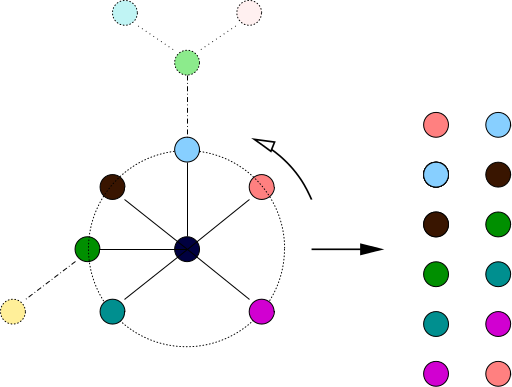
\includegraphics[width=0.7\textwidth]{images/neighborIntervals.png}
\caption{Neighbor intervals of size $2$, from the original paper \cite{harchaoui2007image}.}
\end{figure}

Although we could generalize the previous formula for tree walk kernels easily enough, it would be highly inefficient to evaluate as the number of tree walks of a graph is prohibitively large. In order to make this more efficient, we restrict the set of possible children of a given node in the tree walk to intervals in the cyclic order given by the "planar" embedding of the graph given by the segments of the image.

\begin{figure}[htb!]
\centering
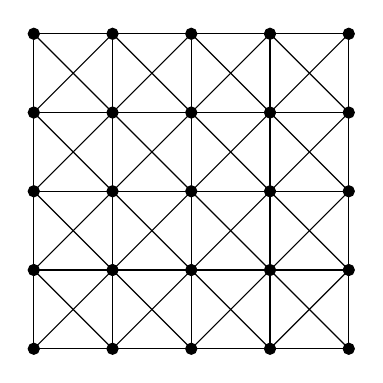
\begin{tikzpicture}[transform shape]
% drawing nodes
\foreach \cx in {1,...,5}{
  \foreach \cy in {1,...,5}{
  	\node[draw,circle,fill=black,inner sep=0.05cm] at (\cx,\cy) {};
  }
}
% drawing edges
\foreach \cx in {1,...,4}{
  \foreach \cy in {1,...,4}{
  	\draw (\cx, \cy) edge ({\cx + 1}, \cy);
  	\draw (\cx, \cy) edge (\cx, {\cy + 1});
  	\draw (\cx, \cy) edge ({\cx + 1}, {\cy + 1});
  	\draw ({\cx + 1}, \cy) edge (\cx, {\cy + 1});
  }
}
\foreach \c in {1,...,4}{
  \draw (\c, 5) edge ({\c + 1}, 5);
  \draw (5, \c) edge (5, {\c + 1});
}
\end{tikzpicture}
\caption{The $8$-connected graph on a $5$ by $5$ image. It has $n = 25$ vertices and $e = 72$ edges, so Euler's planarity criteria $e \leq 3v - 6$ does not hold. Therefore any larger $8$-connected graph must be non planar.}
\label{fig:8connplanar}
\end{figure}

\begin{remark}
At this point, it is necessary to clarify what is meant by the "planar" embedding of the graph, as it is not described in detail in the original paper. It should be noted that the segmentation method in our program does not necessarily yield a planar embedding of the graph using the gravity center of segments, as the segments may be non convex. In fact the graph may not be planar at all using $8$-connectivity for Felzenszwalb's method. Indeed, the $8$-connected graph is not planar for grids larger than $5$ by $5$ pixels by Euler's formula on planar graphs (see \autoref{fig:8connplanar}), and the segmentation is a minor of this graph, which could very well make it non-planar by Wagner's theorem \cite{wagner1937eigenschaft} - such counterexamples were found in practice using Boyer and Myrvold's planarity testing algorithm \cite{boyer2004cutting}. The hue-based merging post-processing step complicates things further, as it ignores the graph structure entirely. If by any chance the resulting graph is planar, then one can use Boyer and Myrvold's planarity testing algorithm to efficiently determine a planar embedding for the graph, but such an embedding may not be representative of the arrangement of segments in the image, and it may not be unique. So in the following we will refer to the "planar" embedding of the graph induced by the segmentation as the embedding given by gravity center of segments, although it may not be planar in the usual definition - hence the quotes around planar.
\end{remark}

Applying this, we can define the \emph{$\alpha$-ary tree walk kernel} of depth $p$ between graphs $G$ and $H$, denoted $k^{p, \alpha}_{\mathcal{T}}$, recursively as follows:

\[
k^{p, \alpha}_{\mathcal{T}}(G,H,r,s) = k(l_G(r), l_H(s)) \sum_{\substack{I \in \mathcal{I}_G^p(r)\\ J \in \mathcal{I}_H^p(s)\\ |I| = |J|}} \prod_{\substack{r' \in I \\ s' \in J}} k^{p - 1, \alpha}_{\mathcal{T}}(G,H,r',s')
\]

Where $k^{1, \alpha}_{\mathcal{T}}(G,H,r,s) = k(l_G(r), l_H(s))$. The final kernel between graphs $G$ and $H$ is then given by summing the recursive kernel for each pairs of root vertices:

\[
k^{p, \alpha}_{\mathcal{T}}(G,H) = \sum_{\substack{r \in V(G)\\ s \in V(H)}} k^{p, \alpha}_{\mathcal{T}}(G,H,r,s)
\]

Using this kernel as a similarity measure between segmentation graphs, we then classify them using the nearest neighbor rule. Although the original paper suggests using color histograms as segment labels, for animation image we found average $L*a*b*$ color to perform as well and to be more efficient. We therefore used a simple Gaussian kernel weighted for segment areas:

\[
k(l_1,l_2) = A_1A_2e^{-\frac{||l_1 - l_2||}{\sigma^2}}
\]

Where $A_1$ and $A_2$ are the areas of segment labelled by $l_1$ and $l_2$ respectively.

\paragraph{Theoretical justification} The idea of comparing graphs for similarity leads us to the problems of graph matching, inexact graph matching and subgraph matching. However these are impractical to solve, and are anyway undesirable - we want to compare graph in a looser fashion. The authors of the original paper therefore combine approaches inspired from text classification and kernel methods to derive the tree walk kernel, and go further to show how the framework of multiple kernel learning can be used to determine the best parameters.

\paragraph{Implementation} Using methods from dynamic programming, we can derive a polynomial time implementation which runs fast in practice. The authors show that, given graphs $G$ and $H$ with maximum degrees $d_G$ and $d_H$ and $n_G$, $n_H$ number of vertices respectively, the algorithm can be implemented to run in $O(p\alpha^2d_Gd_Hn_Gn_H)$ time to compute all $\alpha$-ary tree walk kernels of depth at most $p$.

\paragraph{Results and analysis} The method performed poorly for our purposes, in part because it relies on many parameters which are very difficult to choose.

Further, it seems that the segmentation graphs for animation images have a lot of variations in the smaller substructures of the graph, which makes the relevance of small tree-walks of the graph doubtful for measuring similarity in more global features of the graph. Indeed, computing tree walks of large depth and arity to capture the larger scale features of the graph was found to be impractical. The run time of the algorithm becomes quickly unacceptable for most applications, and is explained by the polynomial complexity of the tree walk kernel computation.

However, it should be noted that the segment matching solution (see \autoref{sec:segmentMatching}), which performed best on our datasets, resembles in many ways the tree walk kernel method, using segment labels and similarity measures between segments to compute an overall similarity for the image, weighing results by segment area. While our method performs better in practice, it lacks a sound theoretical grounding, which could be provided by studying how these two methods relate.

Furthermore, study of the multiple kernel learning method described in the original paper and other works by Bach \cite{bach2004multiple} may give a solution to the problem of choosing the right parameters for the algorithm.

\subsubsection{Segmentation graph spectral classification methods}
The tree walk kernels method performed poorly in part because it relies overly on the smaller variations of the region adjacency graph of the image. In an effort to match graph structure more loosely, we considered the results from spectral graph theory which attempt to analyse graphs through the eigenvalues and eigenvectors of its Laplacian. 

\paragraph{The method} For each segmentation $S$, we consider $m$ features $(f_i : S \rightarrow \mathbb{R}_i^q)_{1 \leq i \leq m}$. For instance, we used average $L^*a^*b^*$ color, gravity center and area of the segment as features. For each feature $f_i$, we compute the $K$-nearest neighbor graph $G_i$ on $S$ with edges weighted by the Gaussian kernel $w(S_u,S_v) = e^{-\frac{||f_i(S_u) - f_i(S_v)||^2}{\sigma_i^2}}$, and its corresponding combinatorial Laplacian  $L_i \in \mathbb{R}^{n \times n}$ where $n$ is the number of segments (see \autoref{sec:laplacians} for definitions).

We then use the method from Wilson, Hancock and Luo \cite{wilson2005pattern} to determine a pattern vector for the graph. To do so, we consider the $k$ eigenvectors $(e_1, ..., e_k)$ corresponding to the $k$ smallest non-zero eigenvalues $(\lambda_1, ..., \lambda_k)$ of $L_i$. 

This method considers the \emph{spectral matrix} $\Phi \in \mathbb{R}^{n \times k}$ which contains the eigenvectors as columns, scaled by the square roots of the eigenvalues.

\[
\Phi = (\sqrt{\lambda_1}e_1 ... \sqrt{\lambda_k}e_k)
\]

Note that the original paper considers all the eigenvectors of the Laplacian. We chose to only use the $k$ first for efficiency and looser graph comparison.
$\Phi$ is well defined as $L_i$ is positive semi definite. Furthermore, $0$ is an eigenvalue of the combinatorial Laplacian for any graph with multiplicity the number of connected components, so this makes clear why we chose to ignore the $0$ eigenvalues - they will only result in a $0$ column for any graph. See \cite{chung1997spectral} for proofs of the elementary properties of the combinatorial Laplacian (and the closely related normalized Laplacian).


The spectral matrix, although it encodes all the information of the $k$ eigenvectors and eigenvalues, cannot directly be used as vector for pattern matching because it is not invariant to vertex permutations on the graph - although the eigenvalues are invariant to such permutations, individual components of the eigenvectors are not. Therefore the authors introduce the \emph{elementary symmetric polynomials} $P = (P_1, ..., P_n)$ to compute $n$ permutation invariant features out of each scaled eigenvectors:

\begin{align*}
P_1(x_1, ..., x_n) &= \sum_{i = 1}^n x_i\\
P_2(x_1, ..., x_n) &= \sum_{i = 1}^n \sum_{j = i + 1}^n x_ix_j\\
... & \\
P_r(x_1, ..., x_n) &= \sum_{0 < i_1 < ... < i_r < n} \prod_{j = 1}^r x_{i_r}\\
... & \\
P_n(x_1, ..., x_n) &= \prod_{i = 1}^n x_i
\end{align*}

So, for each column $\Phi_i = \sqrt{\lambda_i}e_i$ of $\Phi$, we apply each symmetric polynomial to its components to obtain a new vector $E_i \in \mathbb{R}^n$ defined as:

\[
E_i = \begin{pmatrix}
signum(P_1(\Phi_i)) ln(1 + |P_1(\Phi_i)|) \\
... \\
signum(P_n(\Phi_i)) ln(1 + |P_n(\Phi_i)|)
\end{pmatrix}
\] 

The logarithmic scaling is added to adjust the distribution of terms in the polynomials, as suggested in the original paper. Concatenating these vectors for each of the $k$ columns of the spectral matrix, we get a single feature vector $B \in \mathbb{R}^{nk}$. Applying this method to each graph $G_i$ then gives us $m$ feature vectors $(B_i)_{1 \leq i \leq m}$ which we concatenate into the final feature vector $F \in \mathbb{R}^{nmk}$ for the image. We then classify the images by these feature vectors using support vector machines.

We deal with graphs of different size - when the images have different number of segments, which is almost always the case with Felzenszwalb's method - by padding the Laplacian matrix with zeros to match the largest graph in the dataset, as suggested in the original paper.

\paragraph{Theoretical justification}
Works by Wilson, Zhu, Hancock and Luo showed that such spectral methods could be used for graph pattern matching, including image classification through shock graphs \cite{wilson2005pattern}\cite{wilson2008study}. Furthermore, works in graph cut algorithms and application to clustering \cite{ng2002spectral} and segmentation\cite{shi2000normalized}\cite{meila2001random} showed that the eigenvectors of the Laplacian corresponding to smaller eigenvalue encode to some extent sense the global structure of the graph, while ignoring smaller details. We hoped this would allow the method to be robust to variations in animation character images, and encode the information about the global structure of the image.

\paragraph{Implementation}
Computing our $3$ features of interest - average color, gravity center and area of the segments - can be done in one pass over the image and runs in $O(q)$ time where $q$ is the number of pixels in the image. Computing the $K$-nearest neighbor graph for each feature can then be done using an algorithm solving the all nearest neighbor problem, which can be done in $O(Kn\log(n))$ where $n$ is the number of segments in the image \cite{clarkson1983fast}. The resulting graphs are sparse, as the number of edges is at most $K$ times the number of vertices.

For each graph, we can then compute its Laplacian using a sparse matrix data structure in $O(n)$ time by sparsity of the graph and using an adjacency list data structure. We can compute the multiplicity $l$ of the eigenvalue $0$ by running a connected components detection algorithm on the graph, which runs in $O(n)$ time using a simple depth first search procedure. We can then efficiently compute the $k$ eigenvectors of the Laplacian matrix corresponding to the smallest non zero eigenvalues by computing the $k + l$ smallest eigenvectors using the Lanczos method for sparse symmetric matrices, which can be tuned to run in $O((k + l)n^2)$ time \footnote{
There is little literature on the run time complexity of the Lanczos algorithm. However, being an iterative method, we found in practice that limiting the number of iterations to $n$ yields good enough results. Each iteration being dominated by a sparse matrix by dense vector product which runs in $O(n)$ time, and repeating the process for each of the $k + l$ eigenvectors, it is easy to deduce this run time complexity. However, the specifics of the implementation used - here from the Fortran library Arpack - may introduce more run time for the sake of numerical stability, and optimizations to compute multiple eigenvectors at once are not accounted for, so this may not be a very informative result.
}.

Evaluating all the symmetric polynomials for a single column of $\Phi$ can be implemented in $O(n^2)$ time using the \emph{power symmetric functions} $Q = (Q_1, ..., Q_n)$:

\[
\forall r \in \{1, ..., n\} \quad Q_r(x_1, ..., x_n) = \sum_{i = 1}^n x_i^r
\]

And the Newton-Girard formula:

\[
P_r = \frac{(-1)^{r+1}}{r} \sum_{i = 1}^r (-1)^{i + r}Q_iP_{r - i}
\]


Where $Q_0$ denotes the constant $1$ polynomial. One can first compute all the power symmetric functions in $O(n^2)$ time by accumulating the exponentiation of the terms of the sum from one polynomial to the next. We can then compute all the elementary symmetric polynomials by accumulating the inner sum of the Newton-Girard formula in $O(n^2)$ for a total $O(n^2)$ running time. So evaluating the feature vector for all columns of $\Phi$ takes $O(kn^2)$ run time.

So the procedure to compute the pattern vector for a single image runs in $O(q + (k + l)n^2)$ time.

\paragraph{Results and analysis}
Recognition rates measured using leave one out cross validation on a dataset of $12$ characters results in a $10\%$ recognition rate, which is barely better than random. Other methods based on the eigenvalues and eigenvectors of various Laplacians of graphs on the set of segments were considered, with similar results.

The main issue of this method is that the Laplacian only encodes information about edges in the graph, therefore only contains information about segments relative to other segments in the image. The information about the segments themselves, and more importantly between segments of different images, is largely lost. For animation images, segment labelling information turns out to be more important than the structure of segments in the image.

Further, the theory behind the algorithm is not completely sound. The paper by Wilson, Hancock and Luo does indicate that the vectors obtained are not necessarily very useful for pattern matching, and should go through some form of dimensionality reduction to be embedded in a pattern space \cite{wilson2005pattern}. Indeed, this may solve the problem of graphs of different size to some extent, as padding the Laplacian with zeros effectively adds zeros to the final pattern vector.

\subsubsection{Segment matching method}
\label{sec:segmentMatching}
\begin{figure}[htb!]
\centering
\begin{subfigure}{0.24\textwidth}

\includegraphics[width=\textwidth]{images/rufy_d.png}
\end{subfigure}
\begin{subfigure}{0.24\textwidth}

\includegraphics[width=\textwidth]{images/rufy_original2.png}
\end{subfigure}
\begin{subfigure}{0.24\textwidth}
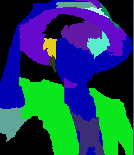
\includegraphics[width=\textwidth]{images/luffy_match1.png}x
\end{subfigure}
\begin{subfigure}{0.24\textwidth}
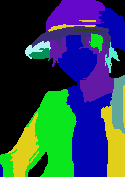
\includegraphics[width=\textwidth]{images/luffy_match2.png}
\end{subfigure}
\caption{Original images (left) and corresponding relation (right). Segments with the same color are matched together.}
\end{figure}

One of the big issues with the previous methods comes from the graphs on the set of segments of a single image not encoding enough information from the image for classification. In an effort to extract more information from the image and to compare the segment information between images directly, we tried to consider how one could match segments between $2$ segmentations, so matched segments could correspond to the same part of the character. This resulted in the following method.

\paragraph{The method} We once again consider some features on the set of segments of the image, namely average $L^*a^*b^*$ color, gravity center and area of the segment. We compute similarity between the segments of $2$ images using a fuzzy control system taking the similarity in features as inputs, and returning an overall similarity of the $2$ segments.

\begin{figure}[htb!]
\centering
\begin{subfigure}{\textwidth}
\centering
\tikzstyle{block} = [draw, fill=blue!20, rectangle, 
    minimum height=6em, minimum width=6em]
\tikzstyle{pinstyle} = [pin edge={to-,thin,black}]
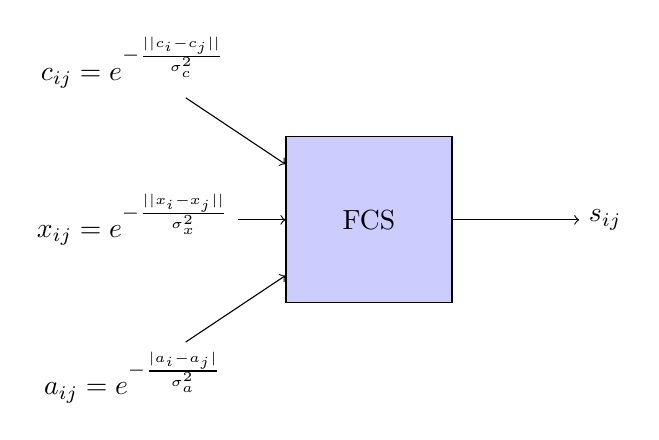
\begin{tikzpicture}[auto, node distance=2cm]
\node (colInput) {$c_{ij} = e^{-\frac{||c_i - c_j||}{\sigma_c^2}}$};
\node [below of=colInput] (posInput) {$x_{ij} = e^{-\frac{||x_i - x_j||}{\sigma_x^2}}$};
\node [below of=posInput] (areaInput) {$a_{ij} = e^{-\frac{|a_i - a_j|}{\sigma_a^2}}$};
\node [block, right of=posInput, node distance=3cm] (fcs) {FCS};
\node [right of=fcs, node distance=3cm] (output) {$s_{ij}$};
\draw [->] (colInput) -- (fcs);
\draw [->] (posInput) -- (fcs);
\draw [->] (areaInput) -- (fcs);
\draw [->] (fcs) -- (output);
\end{tikzpicture}
\caption{Inputs and output.}
\end{subfigure}

\begin{subfigure}{\textwidth}
\centering
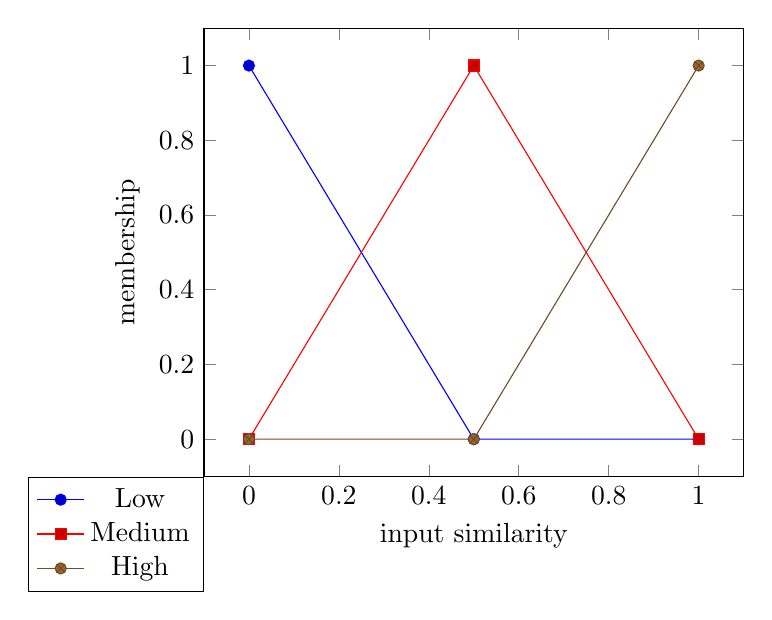
\begin{tikzpicture} 
\begin{axis}[xlabel=input similarity,ylabel=membership,
legend style={
at={(0,0)},
anchor=north east}]
\addplot coordinates {(0,1) (0.5, 0) (1, 0)};
\addlegendentry{Low}
\addplot coordinates {(0,0) (0.5, 1) (1, 0)};
\addlegendentry{Medium}
\addplot coordinates {(0,0) (0.5,0) (1, 1)};
\addlegendentry{High}
\end{axis}
\end{tikzpicture}
\caption{Membership functions for inputs.}
\end{subfigure}

\begin{subfigure}{\textwidth}
\centering
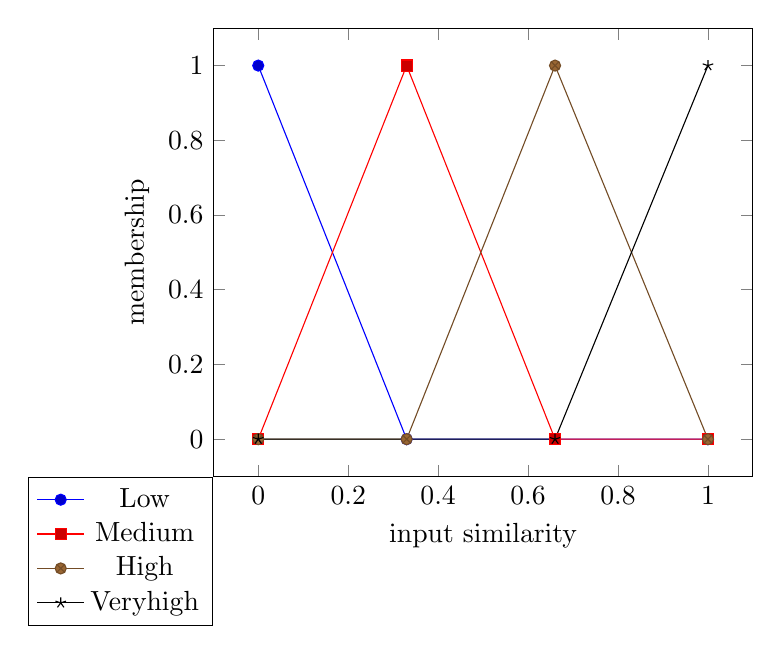
\begin{tikzpicture}
\begin{axis}[xlabel=input similarity,ylabel=membership,
legend style={
at={(0,0)},
anchor=north east}]
\addplot coordinates {(0,1) (0.33, 0) (1, 0)};
\addlegendentry{Low}
\addplot coordinates {(0,0) (0.33, 1) (0.66, 0) (1, 0)};
\addlegendentry{Medium}
\addplot coordinates {(0,0) (0.33,0) (0.66, 1) (1, 0)};
\addlegendentry{High}
\addplot coordinates {(0,0) (0.66, 0) (1, 1)};
\addlegendentry{Veryhigh}
\end{axis}
\end{tikzpicture}
\caption{Membership functions for output.}
\end{subfigure}
\caption{Fuzzy control system (FCS) for segment similarity. For a segment $i$, $c_i$ denotes its average color, $x_i$ the coordinates of its gravity center, $a_i$ its area in number of pixels. $s_{ij}$ denotes the computed similarity between segments $i$ and $j$.}
\end{figure}